\section{Experiments on Image Source Separation}

\subsection{Image Decomposition}
In this section, we turn to use MMCA to separate two-dimensional data and compare the result with the standard ICA source separation techniques. \\

In Figure \ref{segmentation_Im} (a) are two source signals, one of which is oscillating textures while another is  a `boy' image. Curvelet transform is selected as the dictionary for source 1 and discrete consine transform is selected for source 2. This is similar to adpot the idea of a double sparse dictionary therefore we can decompose the mixtures into cartoon and texture. Figure \ref{segmentation_Im} (c) illustrates the separated image using MCA under the presence of 20dB gaussian noise. It can be shown that MCA is able to split the texture and cartoon parts. However, the reconstruction quality of the `boy' image using curvelet dictionary in MCA does not give satisfactory result though. We think the decomposition presenting in the dictionary domain may not be extremely sparse, as some of the mixtures can still be seen in the output image. \\

Note that the MCA algorithm, unlike BSS methods, only takes one single combination of sources ($m = 1$). Now we extend the observed mixtures to a multichannel case and BSS techniques applies. The correlation coefficient between two sources are only 0.07. Hence the independence assumption for ICA methods is valid here. We create four mixtures from two source images.
\ref{segmentation_Im} (d) shows that MMCA is clearly able to efficiently separate the original source images, achieving better visual results than FastICA in (b). Quantitatively, Figure \ref{segmen_1} shows the correlation between the original sources and those estimated. As the data noise variance increase, 
MMCA (dashed line) clearly achieves better estimation quality and shows clear robustness compared to non de-noised ICA methods. In addition, one can note that both JADE and FastICA provides similar performance.\\

Figure \ref{segmen_1} plots the matrix estimation error is defined as $||\mathbf{I_n} - P\tilde{\mathbf{A}}^{+}\mathbf{A} ||$, after elimination the effect of the permutation and scale indeterminacy. Contrasting with standard ICA methods, MMCA iteratively estimates the mixing matrix from coarse (i.e., smooth) versions of the sources and thus is not penalized by the presence of noise. As a consequence, MMCA is clearly more robust to noise than standard ICA methods, even under very noisy context \cite{BobinJ_2006Mdas}.\\

The results in this experiment proves that sparsity based methods successfully handle the image segmentation task. Especially under the multichannel case, MMCA significantly outperforms the standard ICA methods in terms of separation quality and robustness.\\

% -------------------------
\begin{figure}[h]
\centering
\subfigure[]{
\begin{minipage}[b]{0.23\linewidth}
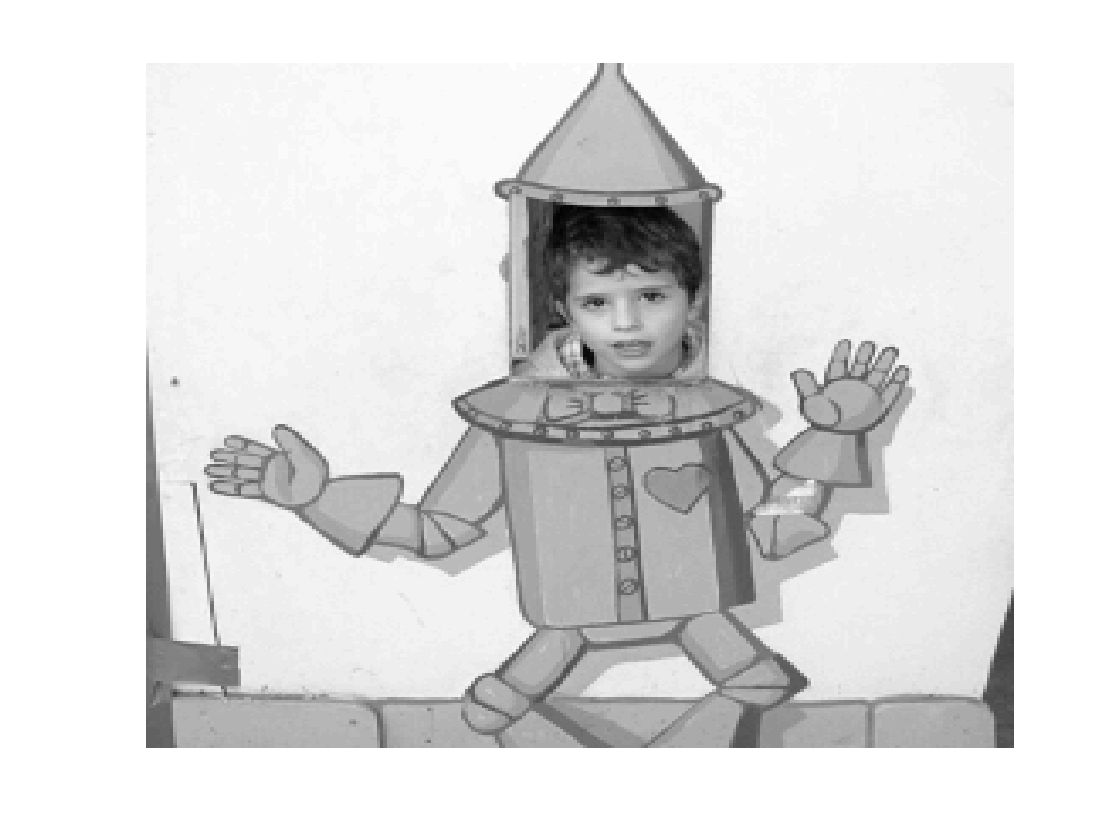
\includegraphics[width=1\linewidth]{images/source1.png}\vspace{1pt}
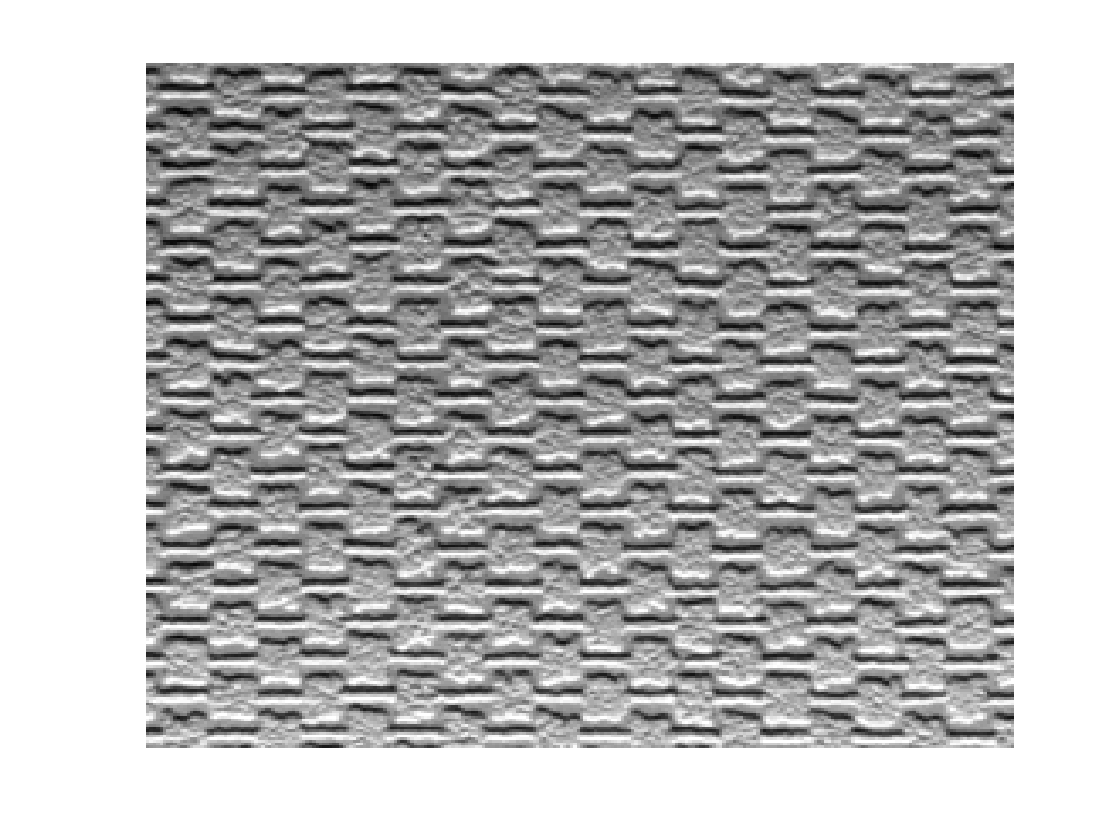
\includegraphics[width=1\linewidth]{images/source2.png}
\end{minipage}}
\subfigure[]{
\begin{minipage}[b]{0.23\linewidth}
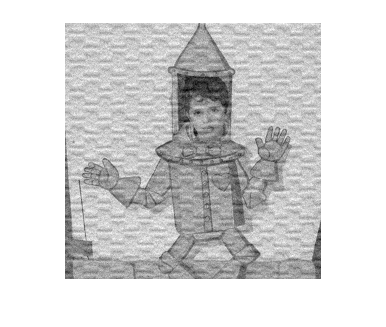
\includegraphics[width=1\linewidth]{images/separated1.png}\vspace{1pt}
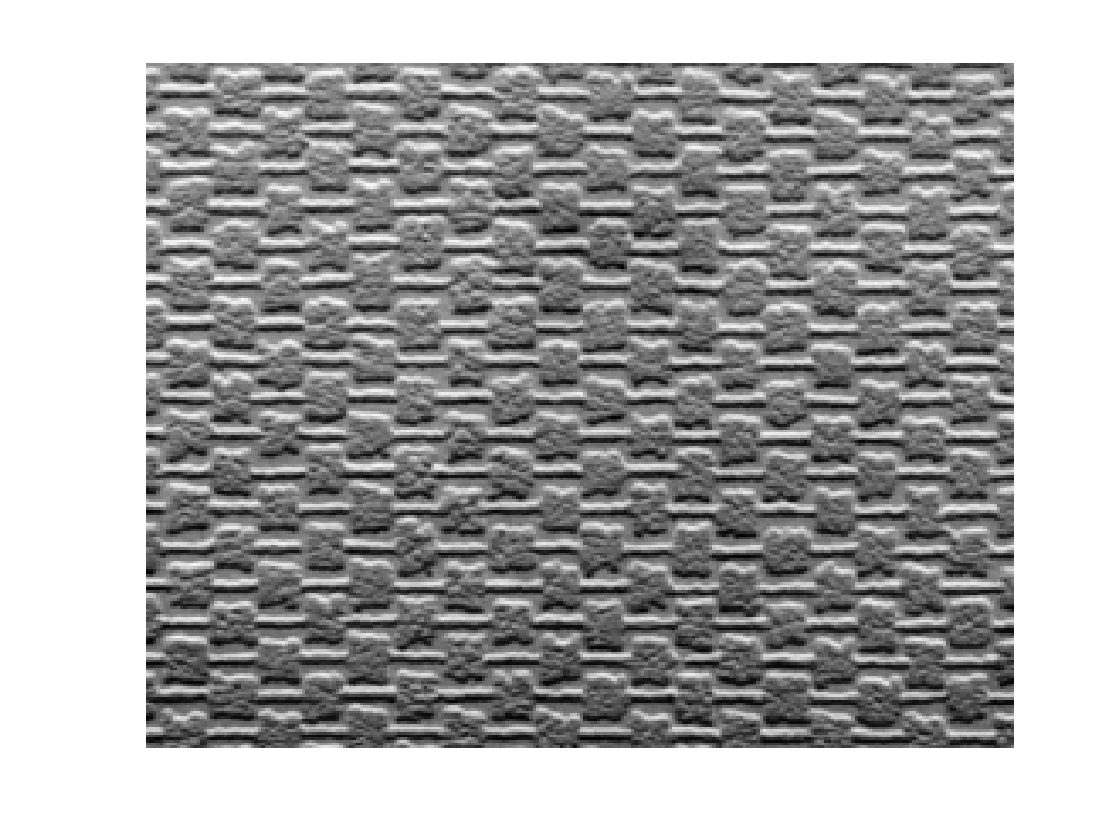
\includegraphics[width=1\linewidth]{images/separated2.png}
\end{minipage}}
\subfigure[]{
\begin{minipage}[b]{0.23\linewidth}
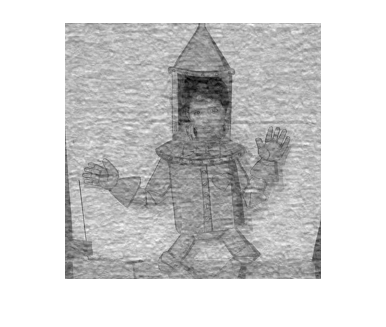
\includegraphics[width=1\linewidth]{images/MCA_Cartoon.png}\vspace{1pt}
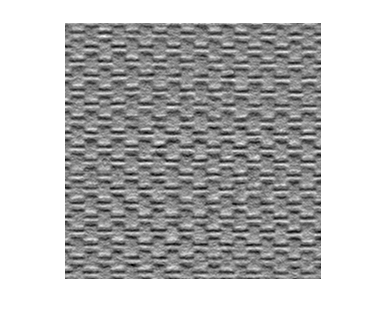
\includegraphics[width=1\linewidth]{images/MCA_Texture.png}
\end{minipage}} 
\subfigure[]{
\begin{minipage}[b]{0.23\linewidth}
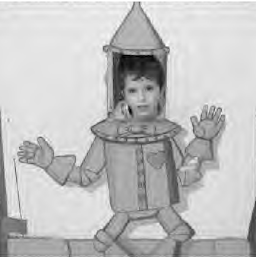
\includegraphics[width=1\linewidth]{images/mmca_cartoon.png}\vspace{1pt}
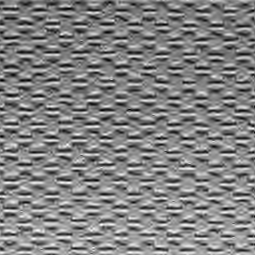
\includegraphics[width=1\linewidth]{images/mmca_texture.png}
\end{minipage}}
\caption{Experiment1: Image segmentation (PSNR = 20dB); \textbf{(a)}: Original sources; \textbf{(b)}: FastICA outputs; \textbf{(c)}: MCA outputs; \textbf{(d)}: MMCA outputs}
\label{segmentation_Im}
\end{figure}
% -------------------------


\begin{figure}[!tbp]
\centering
\begin{minipage}[b]{0.49\textwidth}
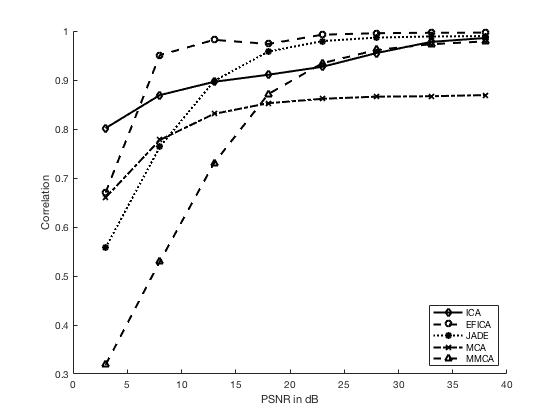
\includegraphics[width=\textwidth]{images/corr_plot_seg.png}
\caption{Evolution of the correlation coefficient between original and estimated sources as the noise variance varies.}
\label{segmen_1}
\end{minipage}
\begin{minipage}[b]{0.49\textwidth}
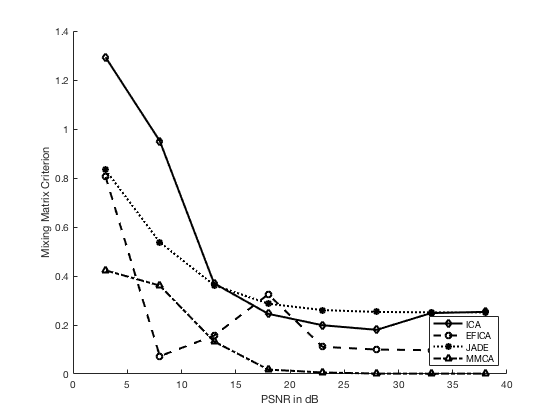
\includegraphics[width=\textwidth]{images/mmc_plot_seg.png}
\caption{Evolution of the mixing matrix criterion (after indeterminacy corrected) as the noise variance varies.}
\end{minipage}
\label{segmen_2}
\label{imapint1}
\end{figure}

\subsection{Blind Image Source Separation}

GMCA is supposed to achieve better separation quality when the mixing sources have similar morphologies. In this experiment, we use two scenery photo and compare GMCA with FastICA. Figure X (c) and (d) are two mixed signals. The result shows that both the two methods achieves good separation quality, but GMCA is slightly better. \\
In the robustness test, we impose guassian noise from 0dB to 30 dB. Figure X (c) and (d) are two mixed signals contaminated by 30dB noise. We can merely identify the original source from (e) and (f), but (c) and (d) using GMCA still gives acceptable result. It can also be shown in Figure X that noise has a greater effect on FastICA than GMCA. 


% ------------
\begin{figure*}
\centering
\subfigure[]{
\begin{minipage}[b]{0.23\linewidth}
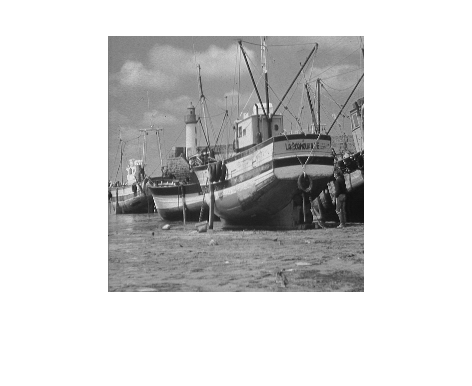
\includegraphics[width=1\linewidth]{images/boat_ori.png}\vspace{4pt}
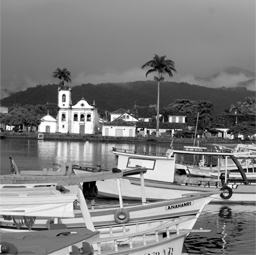
\includegraphics[width=1\linewidth]{images/paraty_ori.png}\vspace{4pt}
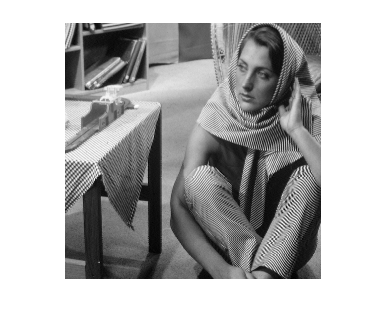
\includegraphics[width=1\linewidth]{images/barbara_ori.png}\vspace{4pt}
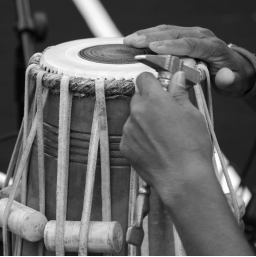
\includegraphics[width=1\linewidth]{images/pakhawaj_ori.png}
\end{minipage}}
\subfigure[]{
\begin{minipage}[b]{0.23\linewidth}
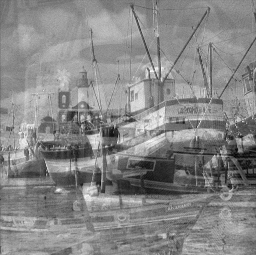
\includegraphics[width=1\linewidth]{images/efica_out1.png}\vspace{4pt}
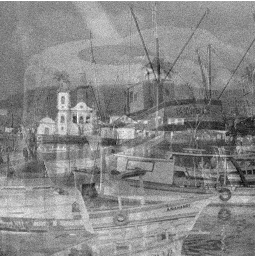
\includegraphics[width=1\linewidth]{images/efica_out2.png}\vspace{4pt}
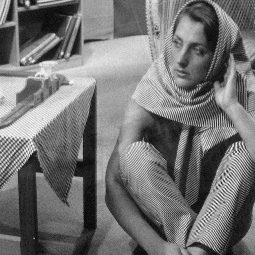
\includegraphics[width=1\linewidth]{images/efica_out3.png}\vspace{4pt}
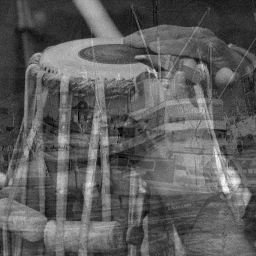
\includegraphics[width=1\linewidth]{images/efica_out4.png}
\end{minipage}}
\subfigure[]{
\begin{minipage}[b]{0.23\linewidth}
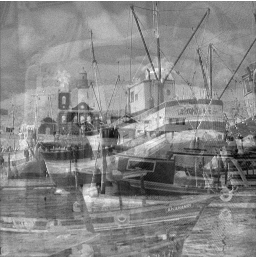
\includegraphics[width=1\linewidth]{images/jade_out1.png}\vspace{4pt}
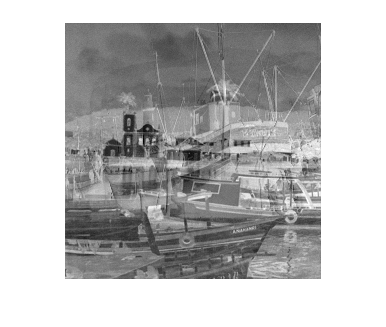
\includegraphics[width=1\linewidth]{images/jade_out2.png}\vspace{4pt}
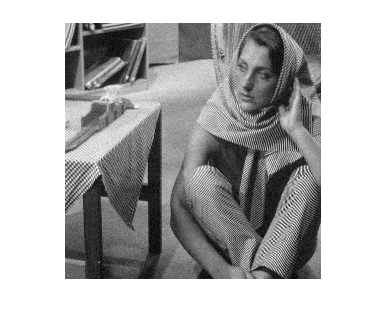
\includegraphics[width=1\linewidth]{images/jade_out3.png}\vspace{4pt}
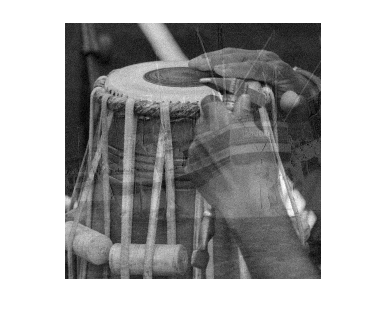
\includegraphics[width=1\linewidth]{images/jade_out4.png}
\end{minipage}}
\subfigure[]{
\begin{minipage}[b]{0.23\linewidth}
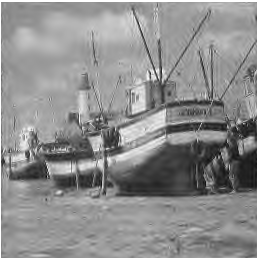
\includegraphics[width=1\linewidth]{images/gmca_out1.png}\vspace{4pt}
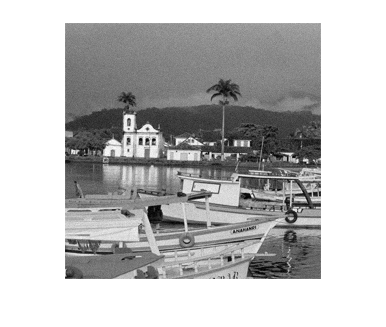
\includegraphics[width=1\linewidth]{images/gmca_out2.png}\vspace{4pt}
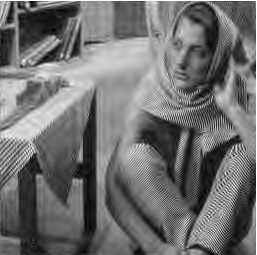
\includegraphics[width=1\linewidth]{images/gmca_out3.png}\vspace{4pt}
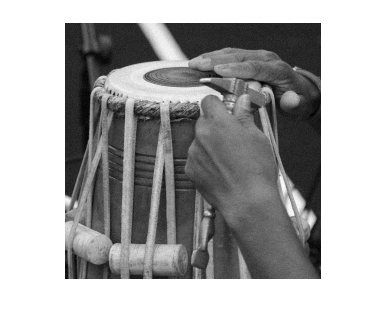
\includegraphics[width=1\linewidth]{images/gmca_out4.png}
\end{minipage}}
\caption{Experiment2: image separation; \textbf{(a)}:Original image sources; \textbf{(b)}:EFICA outputs; \textbf{(c)}:JADE outputs; \textbf{(d)}:GMCA outputs }
\end{figure*}
% ------------ 
\begin{figure}[!tbp]
\centering
\begin{minipage}[b]{0.49\textwidth}
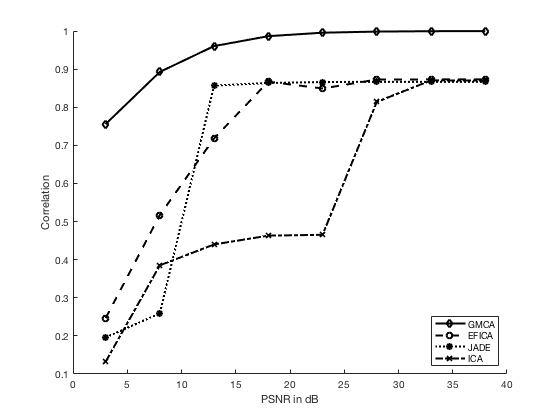
\includegraphics[width=\textwidth]{images/image_separation1.png}
\caption{Evolution of the correlation coefficient between original and estimated sources as the noise variance varies.}
\end{minipage}
\begin{minipage}[b]{0.49\textwidth}
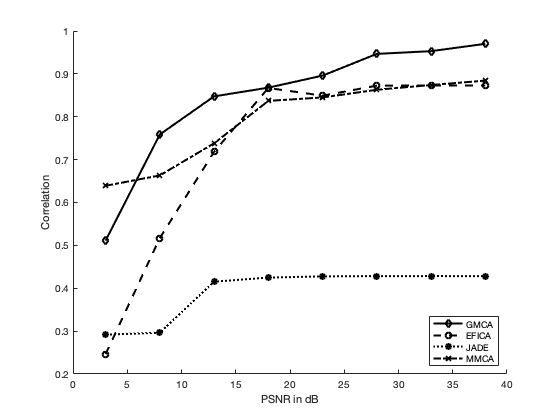
\includegraphics[width=\textwidth]{images/image_separation2.png}
\caption{Evolution of the mixing matrix criterion (after indeterminacy corrected) as the noise variance varies.}
\end{minipage}
\label{plot21}
\end{figure}

\subsection{Blind image separation using adaptive dictionary learning}
In order to obtain enough training samples for dictionary learning, multiple overlapped segments (patches) of the sources are taken. To extract small overlapped patches from the source image. Here, we do not require the prior knowledge of the scaling matrix in front of the true mixing matrix [10], as otherwise required in MMCA and GMCA algorithms.\\

In addition, it is also worth noting that the SparseBSS model, using one dictionary to sparsely represent all the sources will get almost the same performance as using multiple but same-sized dictionaries when the dictionary redundancy d/n is large enough. As a result, it is reasonable to train only one dictionary for all the sources. An obvious advantage of using one dictionary is that the computational cost does not increase when the number of sources increases.\\
\begin{figure}[h]
\centering
\subfigure[]{
\begin{minipage}[b]{0.99\linewidth}
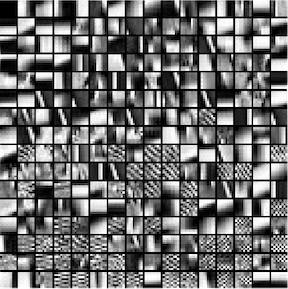
\includegraphics[width=0.23\linewidth]{images/dic1.png}\vspace{4pt}
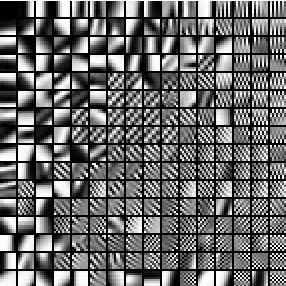
\includegraphics[width=0.23\linewidth]{images/dict3.png}\vspace{4pt}
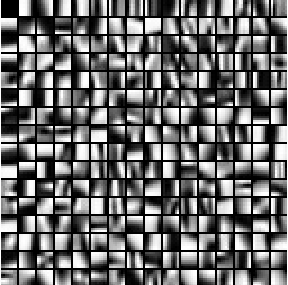
\includegraphics[width=0.23\linewidth]{images/dic2.png}\vspace{4pt}
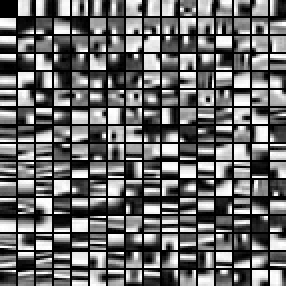
\includegraphics[width=0.23\linewidth]{images/dict4.png}
\end{minipage}}
\subfigure[]{
\begin{minipage}[b]{0.99\linewidth}
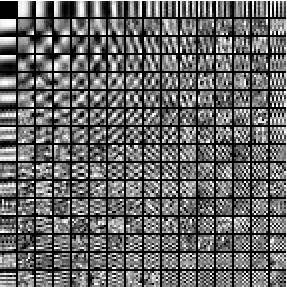
\includegraphics[width=0.23\linewidth]{images/DCT_dict.png}\vspace{4pt}
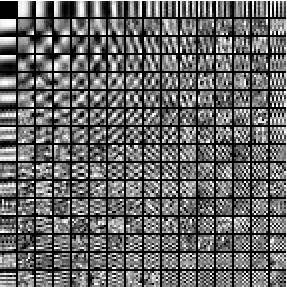
\includegraphics[width=0.23\linewidth]{images/DCT_dict.png}\vspace{4pt}
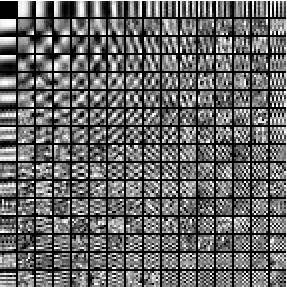
\includegraphics[width=0.23\linewidth]{images/DCT_dict.png}\vspace{4pt}
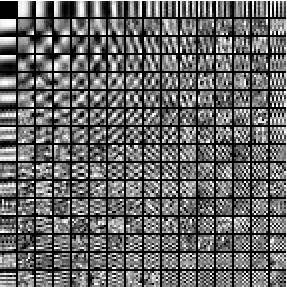
\includegraphics[width=0.23\linewidth]{images/DCT_dict.png}
\end{minipage}}
% \vspace{-0.5cm} 
\caption{Trained Dictionary using K-SVD}
\end{figure}

% --------------------- %
\begin{figure*}
\centering
\subfigure[]{
\begin{minipage}[b]{0.23\linewidth}
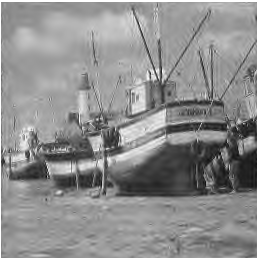
\includegraphics[width=1\linewidth]{images/gmca_out1.png}\vspace{4pt}
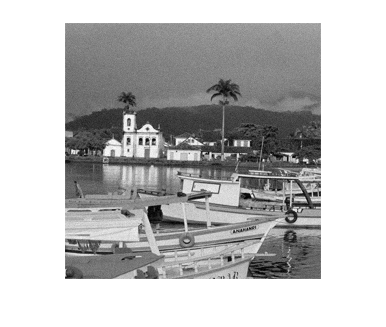
\includegraphics[width=1\linewidth]{images/gmca_out2.png}\vspace{4pt}
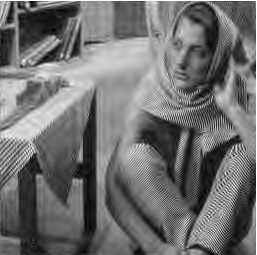
\includegraphics[width=1\linewidth]{images/gmca_out3.png}\vspace{4pt}
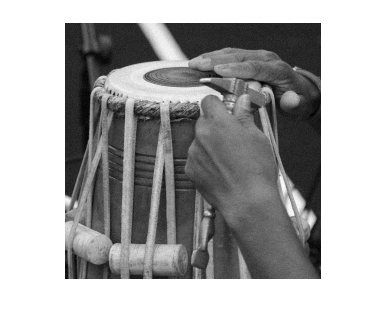
\includegraphics[width=1\linewidth]{images/gmca_out4.png}
\end{minipage}}
\subfigure[]{
\begin{minipage}[b]{0.23\linewidth}
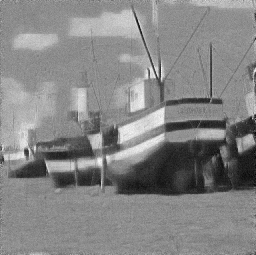
\includegraphics[width=1\linewidth]{images/ammca_out4.png}\vspace{4pt}
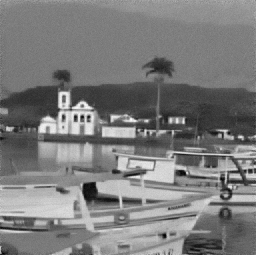
\includegraphics[width=1\linewidth]{images/ammca_out2.png}\vspace{4pt}
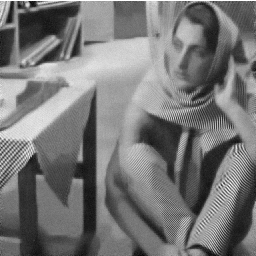
\includegraphics[width=1\linewidth]{images/ammca_out3.png}\vspace{4pt}
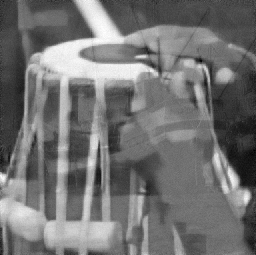
\includegraphics[width=1\linewidth]{images/ammca_out1.png}
\end{minipage}}
\caption{Experiment3: Using adaptive dictionary learning; \textbf{(a)}:Original image sources; \textbf{(b)}:GMCA outputs; \textbf{(c)}:K-SVD+MMCA outputs;}
\end{figure*}